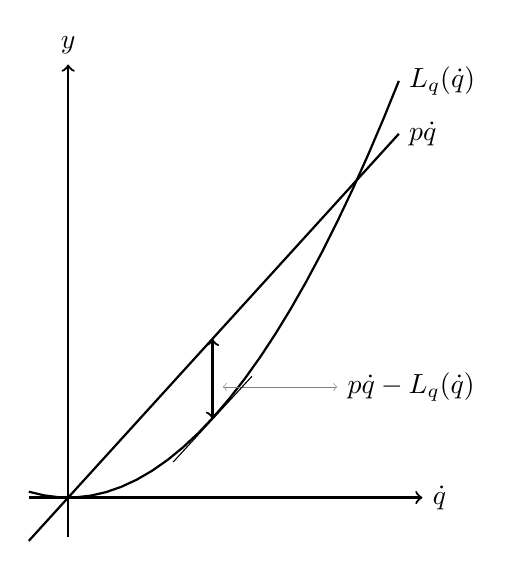
\begin{tikzpicture}
    \draw[->, thick] (-0.5, 0) -- (4.5, 0) node[anchor=west] {$\dot{q}$};
    \draw[->, thick] (0, -0.5) -- (0, 5.5) node[anchor=south] {$y$};
    
    \draw[thick, domain=-0.5:4.2] plot ({\x}, {0.3*\x*\x}) node[anchor=west] {$L_q(\dot{q})$};
    \draw[thick, domain=-0.5:4.2] plot ({\x}, {1.1*\x}) node[anchor = west] {$p\dot{q}$};
    
    \draw[<->, thick] (1.8333, 1) -- (1.8333, 2.01663) node[pos=0.4, pin={[right, xshift=1cm]0:{$p \dot{q} - L_q(\dot{q})$}}] {};
    
    \draw (1.8333, 1) ++(-0.5, -0.549) -- ++(1, 1.089);
    
\end{tikzpicture}